
\newpage % Эта команда начинает новую страницу
\chapter{Очереди}

\section{Однонаправленные очереди}

Очереди представляют структуру данных, работающую по принципу FIFO (first in - first out). Чем раньше был добавлен элемент в коллекцию, тем раньше он из нее удаляется. Это стандартная модель однонаправленной очереди.

Создадим класс, который позволит «складывать» туда объекты в заранее неизвестном количестве и «вынимать» объекты из этой очереди. По сути класс должен иметь три метода:
\begin{enumerate}
\item Положить объект (произвольного класса) в очередь — назовем метод push;
\item Вытащить объект (произвольного класса) из очереди — назовем метод pull;
\item Получить количество объектов в очереди — назовем его size.
\end{enumerate}

Итак, наш класс ObjectQueue будет выглядеть (без реализации, только с методами) вот так:


\begin{lstlisting}
public class ObjectQueue
{
    public void push(Object obj) {
        ...
    }
 
    public Object pull() {
        ...
    }
 
    public int size() {
        ...
    }
}
\end{lstlisting}

Как видите, мы можем положить в очередь объект типа Object, что означает, что мы можем положить туда все, что угодно — класс Object является «проматерью» всех классов, — все классы наследуются в конечном итоге от него.
\section{Стратегия доступа к элементам очереди}

В очереди обычно используются следующие операции:
\begin{enumerate}
\item Enqueue — добавляет элемент из конца очереди.
\item Dequeue — удаляет элемент из начала очереди.
\item Front/Peek — возвращает значение элемента, находящегося перед очередью, без исключения (удаления) элемента из очереди.
\item IsEmpty — проверяет, пуста ли очередь.
\item IsFull — проверяет, заполнена ли очередь.
\item Display — распечатывает все элементы в очереди.
\end{enumerate}

Новые элементы очереди можно добавлять как в начало списка, так и в конец. Важно только, чтобы элементы доставались с противоположного края.

\section{Реализация Priority Queue}

Приоритетная очередь — абстрактная структура данных наподобие стека или очереди, где у каждого элемента есть приоритет. Элемент с более высоким приоритетом находится перед элементом с более низким приоритетом. Если у элементов одинаковые приоритеты, они располагаются в зависимости от своей позиции в очереди. Обычно приоритетные очереди реализуются с помощью куч

Приоритетные очереди поддерживают следующие операции:

\begin{itemize}
\item findMin или findMax — поиск элемента с наибольшим приоритетом,
\item insert или push — вставка нового элемента,
\item extractMin или extractMax — извлечь элемент с наибольшим приоритетом,
\item deleteMin или deleteMax — удалить элемент с наибольшим приоритетом,
\item increaseKey или decreaseKey — обновить значение элемента,
\item merge — объединение двух приоритетных очередей, сохраняя оригинальные очереди,
\item meld — объединение двух приоритетных очередей, разрушая оригинальные очереди,
\item split — разбить приоритную очередь на две части.
\end{itemize}

Следующий сегмент кода создает пустую PriorityQueue, а затем добавляет в очередь несортированные (даже частично не отсортированные) значения:

\begin{lstlisting}
PriorityQueue<Integer> pq = new PriorityQueue<Integer>();

pq.add(69); pq.add(65); pq.add(87); pq.add(79);

pq.add(73); pq.add(84); pq.add(89); pq.add(80);

pq.add(81); pq.add(82); pq.add(85);
\end{lstlisting}

Все эти числа целые. Они взяты из частично отсортированного списка, но в настоящее время они полностью не отсортированы по мере ввода. Элементы в pq теперь частично отсортированы в соответствии с определением приоритетной очереди в Java. %https://andreyex.ru/programmirovanie/java/prioritetnaya-ochered-v-java/

\section{Двунаправленные очереди}

Интерфейс Deque расширяет интерфейс Queue и определяет поведение двунаправленной очереди, которая работает как обычная однонаправленная очередь, либо как стек, действующий по принципу LIFO (последний вошел - первый вышел).

Интерфейс Deque определяет следующие методы:

\begin{itemize}
\item void addLast(E obj): добавляет элемент obj в конец очереди
\item E getFirst(): возвращает без удаления элемент из головы очереди. Если очередь пуста, генерирует исключение NoSuchElementException
\item E getLast(): возвращает без удаления последний элемент очереди. Если очередь пуста, генерирует исключение NoSuchElementException
\item boolean offerFirst(E obj): добавляет элемент obj в самое начало очереди. Если элемент удачно добавлен, возвращает true, иначе - false
\item boolean offerLast(E obj): добавляет элемент obj в конец очереди. Если элемент удачно добавлен, возвращает true, иначе - false
\item E peekFirst(): возвращает без удаления элемент из начала очереди. Если очередь пуста, возвращает значение null
\item E peekLast(): возвращает без удаления последний элемент очереди. Если очередь пуста, возвращает значение null
\item E pollFirst(): возвращает с удалением элемент из начала очереди. Если очередь пуста, возвращает значение null
\item E pollLast(): возвращает с удалением последний элемент очереди. Если очередь пуста, возвращает значение null
\item E pop(): возвращает с удалением элемент из начала очереди. Если очередь пуста, генерирует исключение NoSuchElementException
\item void push(E element): добавляет элемент в самое начало очереди
\item E removeFirst(): возвращает с удалением элемент из начала очереди. Если очередь пуста, генерирует исключение NoSuchElementException
\item E removeLast(): возвращает с удалением элемент из конца очереди. Если очередь пуста, генерирует исключение NoSuchElementException
\item boolean removeFirstOccurrence(Object obj): удаляет первый встреченный элемент obj из очереди. Если удаление произшло, то возвращает true, иначе возвращает false.
\item boolean removeLastOccurrence(Object obj): удаляет последний встреченный элемент obj из очереди. Если удаление произшло, то возвращает true, иначе возвращает false.
\end{itemize}


Таким образом, наличие методов pop и push позволяет классам, реализующим этот элемент, действовать в качестве стека. В тоже время имеющийся функционал также позволяет создавать двунаправленные очереди, что делает классы, применяющие данный интерфейс, довольно гибкими.

\section{Реализация ArrayList, Array Deque}
\subsection{ArrayList}
Для создания простых списков применяется интерфейс List, который расширяет функциональность интерфейса Collection. Некоторые наиболее часто используемые методы интерфейса List:

\begin{itemize}
\item void add(int index, E obj): добавляет в список по индексу index объект obj
\item boolean addAll(int index, Collection<? extends E> col): добавляет в список по индексу index все элементы коллекции col. Если в результате добавления список был изменен, то возвращается true, иначе возвращается false
\item E get(int index): возвращает объект из списка по индексу index
\item int indexOf(Object obj): возвращает индекс первого вхождения объекта obj в список. Если объект не найден, то возвращается -1
\item int lastIndexOf(Object obj): возвращает индекс последнего вхождения объекта obj в список. Если объект не найден, то возвращается -1
\item ListIterator<E> listIterator (): возвращает объект ListIterator для обхода элементов списка
\item static <E> List<E> of(элементы): создает из набора элементов объект List
\item E remove(int index): удаляет объект из списка по индексу index, возвращая при этом удаленный объект
\item E set(int index, E obj): присваивает значение объекта obj элементу, который находится по индексу index
\item void sort(Comparator<? super E> comp): сортирует список с помощью компаратора comp
\item List<E> subList(int start, int end): получает набор элементов, которые находятся в списке между индексами start и end
\end{itemize}

В следующем примере рассмотрим создание объекта класса ArrayList и добавление в него элементов с помощью указанных выше методов:

\begin{lstlisting}
public class ArrayListAddDemo {
    public static void main(String[] args) {
        List<String> arrayList = new ArrayList<>();

        System.out.println("Initial size arrayList: "
                + arrayList.size());

        arrayList.add("C");
        arrayList.add("A");
        arrayList.add("E");
        arrayList.add("B");
        arrayList.add("D");
        arrayList.add("F");
        arrayList.add("F");
        arrayList.add(1, "A2");
        arrayList.set(0, "C2");

        System.out.println("arrayList size after adding: "
                + arrayList.size());
        System.out.println("arrayList content: " + arrayList);
        System.out.println(arrayList.get(0));
    }
}
\end{lstlisting}

\subsection{ArrayDeque}

В Java очереди представлены рядом классов. Одни из низ - класс ArrayDeque<E>. Этот класс представляют обобщенную двунаправленную очередь, наследуя функционал от класса AbstractCollection и применяя интерфейс Deque.

В классе ArrayDeque определены следующие конструкторы:
\begin{itemize}
\item ArrayDeque(): создает пустую очередь
\item ArrayDeque(Collection<? extends E> col): создает очередь, наполненную элементами из коллекции col
\item ArrayDeque(int capacity): создает очередь с начальной емкостью ca-\newline pacity. Если мы явно не указываем начальную емкость, то емкость по умолчанию будет равна 16
\end{itemize}

Пример использования класса ArrayDeque:

\begin{lstlisting}
public class ArrayDequeExample {
    public static void main(String[] args) {
        Deque<String> stack = new ArrayDeque<>();
        Deque<String> queue = new ArrayDeque<>(2);
        stack.push("A");
        stack.push("B");
        stack.push("C");
        stack.push("D");
        while (!stack.isEmpty()) {
            System.out.print(stack.pop() + " ");
        }
        System.out.println();

        queue.add("A");
        queue.add("B");
        queue.add("C");
        queue.add("D");
        while (!queue.isEmpty()) {
            System.out.print(queue.remove() + " ");
        }
    }
} 
\end{lstlisting}

\section{Анализ и сложность операций производимых над элементами очереди}


\begin{itemize}
\item Метод Enqueue

Поведение: Добавляет элемент в очередь.
Сложность: O(1).
\item Метод Dequeue

Поведение: Удаляет первый помещенный элемент из очереди и возвращает его. Если очередь пустая, кидает InvalidOperationException.
Сложность: O(1).
\item Метод Peek

Поведение: Возвращает элемент, который вернет следующий вызов метода Dequeue. Очередь остается без изменений. Если очередь пустая, кидает InvalidOperationException.
Сложность: O(1).
\item Метод Count

Поведение: Возвращает количество элементов в очереди или 0, если очередь пустая.
Сложность: O(1).
\end{itemize}

O(1) можно прочитать как «сложность порядка 1» (order 1), или «алгоритм выполняется за постоянное/константное время» (constant time). O(1) алгоритмы самые эффективные.
%https://habr.com/ru/articles/444594/

\chapter{Карты}

В Java словари, также называемые картами и отображениями, реализованы классами HashMap, TreeMap (через интерфейс SortedMap), Hashtable (хэш-таблица), LinkedHashMap. Словарь представляет собой набор пар ключ-значение. При этом ключ в пределах словаря должен быть уникальным.

Добавление элемента в словарь выполняется методом put(key, value), получение значения по ключу – get(key).

С помощью методов entrySet(), keySet() и values() получают множества соответственно пар, ключей, либо значений. Их можно преобразовать в списки, например, передав в конструктор List'а или методом addAll().

\begin{lstlisting}
import java.util.ArrayList;
import java.util.HashMap;
 
public class MapTest {
    public static void main(String[] args) {
 
        HashMap<String, String> map =
                new HashMap<>();
        map.put("One", "Odin");
        map.put("Two", "Dva");
        map.put("Three", "Tri");
        System.out.println(map);
 
        System.out.println(map.entrySet());
        System.out.println(map.keySet());
        System.out.println(map.values());
 
        ArrayList<String> val =
                new ArrayList<>(map.values());
        System.out.println(val);
 
        ArrayList<HashMap.Entry> entries =
                new ArrayList<>(map.entrySet());
        System.out.println(entries);
        for (HashMap.Entry entry : entries) {
            System.out.println(entry.getKey());
        }
 
        ArrayList<String> keys = new ArrayList<>();
        keys.addAll(map.keySet());
        System.out.println(keys);
    }
}
\end{lstlisting}

Результат:

\begin{lstlisting}
{One=Odin, Two=Dva, Three=Tri}
[One=Odin, Two=Dva, Three=Tri]
[One, Two, Three]
[Odin, Dva, Tri]
[Odin, Dva, Tri]
[One=Odin, Two=Dva, Three=Tri]
One
Two
Three
[One, Two, Three]
\end{lstlisting}

В классе HashMap есть внутренний класс Entry, объекты которого хранят атрибуты одной пары.

Другие часто используемые методы Map: containsKey(key) – проверка наличия ключа, containsValue(value) – проверка наличия значения, remove(key) – удаление элемента по ключу. %https://younglinux.info/java/map

\section{Анализ интерфейса Map}

Map — это структура данных, которая содержит набор пар “ключ-значение”. По своей структуре данных напоминает словарь, поэтому ее часто так и называют. В то же время, Map является интерфейсом, и в стандартном jdk содержит основные реализации: Hashmap, LinkedHash- \newline Map, Hashtable, TreeMap. Все ключи уникальные в рамках объекта Map. Такие коллекции облегчают поиск элемента, если нам известен ключ - уникальный идентификатор объекта.

Следует отметить, что в отличие от других интерфейсов, которые представляют коллекции, интерфейс Map НЕ расширяет интерфейс \newline Collection.

\section{Структура карты, итерация по элементам карты}

Класс HashMap использует хеш-таблицу для хранения карточки, обеспечивая быстрое время выполнения запросов get() и put() при больших наборах. Класс реализует интерфейс Map (хранение данных в виде пар ключ/значение). Ключи и значения могут быть любых типов, в том числе и null. При этом все ключи обязательно должны быть уникальны, а значения могут повторяться. Данная реализация не гарантирует порядка элементов.

Общий вид HashMap:

\begin{lstlisting}
// K - Key, V - Value
class HashMap<K, V>
\end{lstlisting}

Объявить можно следующим образом:

\begin{lstlisting}
Map<String, Integer> hashMap = new HashMap<String, Integer>();
// or
Map<String, String> hashMap = new HashMap<String, String>();
\end{lstlisting}

%https://developer.alexanderklimov.ru/android/java/hashmap.php

Поскольку карта не расширяет Collection интерфейс, у него нет собственного итератора. С Set расширяет Collection интерфейс, мы можем получить итератор для набора ключей, возвращаемых keySet(). Теперь мы можем легко обработать каждый ключ, используя простой цикл while, как показано ниже:

\begin{lstlisting}
Iterator<K> itr = map.keySet().iterator();
while (itr.hasNext())
{
    K key = itr.next();
    V value = map.get(key);
 
    System.out.println(key + "=" + value);
}
\end{lstlisting}

Мы также можем использовать forEachRemaining() метод, который является последним дополнением к Iterator интерфейс в Java 8 и выше. Он выполняет данное действие для каждого оставшегося элемента, пока все элементы не будут обработаны.

\begin{lstlisting}
// using a lambda expression
map.keySet()
    .iterator()
    .forEachRemaining(key -> System.out.println(key + "=" + map.get(key)));
\end{lstlisting}

%https://www.techiedelight.com/ru/iterate-map-using-keyset-java/

\section{Реализация интерфейса Map}

Map является интерфейсом, и в стандартном jdk содержит основные реализации: Hashmap, LinkedHashMap, Hashtable, TreeMap. 

\subsection{HashMap}

Класс HashMap в Java использует хэш-таблицу для реализации интерфейса Map. Это позволяет времени для выполнения основных операций, таких как get () и put (), оставаться постоянным даже для больших множеств. Следующая программа демонстрирует работу нескольких методов, поддерживаемых HashMap в Java:

\begin{lstlisting}
public class HashMapDemo {

   public static void main(String args[]) {
   
      // creating hash map
      HashMap hm = new HashMap();
      
      hm.put("Zarya", new Double(3434.34));
      hm.put("Mark", new Double(123.22));
      hm.put("Aian", new Double(1378.00));
      hm.put("Daisy", new Double(99.22));
      hm.put("Michael", new Double(-19.08));
      
      // getting a type of element
      Set set = hm.entrySet();
      
      // getting iterator
      Iterator i = set.iterator();
      
      // displaying elements
      while(i.hasNext()) {
         Map.Entry me = (Map.Entry)i.next();
         System.out.print(me.getKey() + ": ");
         System.out.println(me.getValue());
      }
      System.out.println();
      
      // deposit 1000 to Zarya's account
      double balance = ((Double)hm.get("Zarya")).doubleValue();
      hm.put("Zarya", new Double(balance + 1000));
      System.out.println("Zarya's new balance: " + hm.get("Zarya"));
   }
}
\end{lstlisting}

Получим следующий результат:

\begin{lstlisting}
Daisy: 99.22
Aian: 1378.0
Zarya: 3434.34
Michael: -19.08
Mark: 123.22

Zarya's new balance: 4434.34
\end{lstlisting}


\subsection{LinkedHashMap}
Класс LinkedHashMap расширяет HashMap и поддерживает связанный список записей на Map в том порядке, в котором они были вставлены. Это позволяет итерации ввода-вывода по Map. То есть при итерировании LinkedHashMap элементы будут возвращены в том порядке, в котором они были вставлены. Следующая программа демонстрирует работу нескольких методов, поддерживаемых коллекцией LinkedHashMap в Java:

\begin{lstlisting}
public class LinkedHashMapDemo {

   public static void main(String args[]) {
      // creating hash map
      LinkedHashMap lhm = new LinkedHashMap();
      
      // putting elements in map
      lhm.put("Zarina", new Double(3434.34));
      lhm.put("Mark", new Double(123.22));
      lhm.put("Andrei", new Double(1378.00));
      lhm.put("Denis", new Double(99.22));
      lhm.put("Michael", new Double(-19.08));
      
      // getting the type of elements
      Set set = lhm.entrySet();
      
      // receiving iterator
      Iterator i = set.iterator();
      
      // displaying elements
      while(i.hasNext()) {
         Map.Entry me = (Map.Entry)i.next();
         System.out.print(me.getKey() + ": ");
         System.out.println(me.getValue());
      }
      System.out.println();
      
      // deposit 1000 to Zarina's account
      double balance = ((Double)lhm.get("Zarina")).doubleValue();
      lhm.put("Zarina", new Double(balance + 1000));
      System.out.println("Zarina's new balance: " + lhm.get("Zarina"));
   }
}
\end{lstlisting}

Получим следующий результат:

\begin{lstlisting}
Zarina: 3434.34
Mark: 123.22
Andrei: 1378.0
Denis: 99.22
Michael: -19.08

Zarina's new balance: 4434.34
\end{lstlisting}

\subsection{HashTable}

Как и HashMap, в Java Hashtable хранит пары ключей/значений в хэш-таблице. Используя Hashtable, вы указываете объект, который используется как ключ, и значение, которое вы ходите связать с этим ключом. Этот ключ затем хэшируется, а полученный хэш-код используется как индекс, в котором значение хранится в таблице. Следующая программа показывает несколько методов, поддерживаемых структурой данных Hashtable в Java:

\begin{lstlisting}
public class HashTableDemo {

   public static void main(String args[]) {
      // creating hash table
      Hashtable balance = new Hashtable();
      Enumeration names;
      String str;
      double bal;

      balance.put("Masha", new Double(3434.34));
      balance.put("Michael", new Double(123.22));
      balance.put("Oleg", new Double(1378.00));
      balance.put("Denis", new Double(99.22));
      balance.put("Anton", new Double(-19.08));

      // shows all balances in a hash table
      names = balance.keys();
      
      while(names.hasMoreElements()) {
         str = (String) names.nextElement();
         System.out.println(str + ": " + balance.get(str));
      }        
      System.out.println();
      
      // deposit 1,000 into Masha's account
      bal = ((Double)balance.get("Masha")).doubleValue();
      balance.put("Masha", new Double(bal + 1000));
      System.out.println("Masha's new balance: " + balance.get("Masha"));
   }
}
\end{lstlisting}

Получим следующий результат:

\begin{lstlisting}
Anton: -19.08
Masha: 3434.34
Michael: 123.22
Denis: 99.22
Oleg: 1378.0

Masha's new balance: 4434.34
\end{lstlisting}

\subsection{TreeMap}

TreeMap в Java реализует интерфейс Map, используя дерево. TreeMap обеспечивает эффективное средство хранения пар ключ/значение в отсортированном порядке и позволяет быстро извлекать данные. Следует отметить, что, в отличие от хэш-карты, карта деревьев гарантирует, что ее элементы будут отсортированы в порядке возрастания ключа. Следующая программа демонстрирует работу нескольких методов, поддерживаемых TreeMap в Java:

\begin{lstlisting}
public class TreeMapDemo {

   public static void main(String args[]) {
      // creating hash map
      TreeMap tm = new TreeMap();
      
      // putting items on the map
      tm.put("Zarya", new Double(3434.34));
      tm.put("Mark", new Double(123.22));
      tm.put("Aian", new Double(1378.00));
      tm.put("Daisy", new Double(99.22));
      tm.put("Michael", new Double(-19.08));
      
      // receiving types of elements
      Set set = tm.entrySet();
      
      // getting an iterator
      Iterator i = set.iterator();
      
      // displaying elements
      while(i.hasNext()) {
         Map.Entry me = (Map.Entry)i.next();
         System.out.print(me.getKey() + ": ");
         System.out.println(me.getValue());
      }
      System.out.println();
      
      // deposit 1000 to Zarya's account
      double balance = ((Double)tm.get("Zarya")).doubleValue();
      tm.put("Zarya", new Double(balance + 1000));
      System.out.println("Zarya's new balance: " + tm.get("Zarya"));
   }
}
\end{lstlisting}

Получим следующий результат:

\begin{lstlisting}
Aian: 1378.0
Daisy: 99.22
Mark: 123.22
Michael: -19.08
Zarya: 3434.34

Zarya's new balance: 4434.34
\end{lstlisting}
%https://proglang.su/java

\chapter{Типы потоков ввода/вывода. Основные классы Java для работы с файловой системой}
\section{Библиотеки ввода/вывода java.io и java.nio}

Отличительной чертой многих языков программирования является работа с файлами и потоками. В Java основной функционал работы с потоками сосредоточен в классах из пакета java.io. 

java.nio — это библиотека, представленная в Java 1.4. Java NIO с момента своего запуска предоставила альтернативный способ обработки операций ввода-вывода и сетевых транзакций. Он считается альтернативой библиотекам Java Networking и Java IO. Java NIO была разработана с целью сделать транзакции для ввода и вывода асинхронными и неблокирующими. Концепция блокирующего и неблокирующего ввода-вывода объясняется в следующих разделах.

Основные отличия между Java IO и Java NIO:

\begin{figure}[h]
\centering
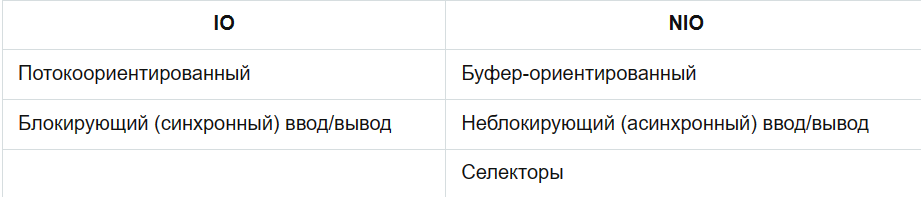
\includegraphics[width=0.8\linewidth]{images/pic/pic20-1.png}
\label{fig:mpr}
\end{figure}

Основное отличие между двумя подходами к организации ввода/вывода в том, что Java IO является потокоориентированным, а Java NIO – буфер-ориентированным.

Потокоориентированный ввод/вывод подразумевает чтение/запись из потока/в поток одного или нескольких байт в единицу времени поочередно. Данная информация нигде не кэшируются. Таким образом, невозможно произвольно двигаться по потоку данных вперед или назад. Если нужно произвести подобные манипуляции, потребуется сначала кэшировать данные в буфере.

\section{Основные классы потоков и их декораторы}

В Java потоки (или нити) являются средством параллельного исполнения кода. Они позволяют запускать несколько частей программы одновременно и, таким образом, ускорять выполнение задач.

Основные классы потоков в Java:

\begin{itemize}
\item Thread - класс, представляющий поток исполнения. Он наиболее часто используется в Java для создания потоков.
\item Runnable - интерфейс, который предоставляет метод run(), реализуя который, можно запускать поток.
\item Executors - класс, предоставляющий пул потоков для выполнения асинхронных задач. Он позволяет управлять количеством потоков, выполняющих задачи, и предоставляет различные методы для выполнения задач.
\item Callable - интерфейс, который похож на Runnable, но возвращает значение типа T после выполнения метода call().
\end{itemize}

Классы потоков в Java также могут быть декорированы с помощью различных аннотаций. Например:

\begin{itemize}
\item @Thread - аннотация, которая позволяет создать поток с помощью ExecutorService. Она позволяет управлять количеством потоков, выполняющих задачи, и задавать приоритеты для каждого потока.
\item @Synchronized - аннотация, которая позволяет блокировать доступ к общим ресурсам, таким как переменные или методы, для избежания состояния гонки (race condition).
\item @Asynchronous - аннотация, которая позволяет выполнить асинхронную задачу в отдельном потоке. Она автоматически создает новый поток для выполнения задачи, что позволяет избежать блокировки основного потока исполнения.
\item @Future - аннотация, которая позволяет получить результат выполнения асинхронной задачи в виде объекта типа Future. Это позволяет продолжить работу основного потока исполнения, пока асинхронная задача не завершится.
\end{itemize}

\section{Класс для работы с файловой системой File}

Класс File предоставляет удобный интерфейс для работы с файловой системой, позволяя создавать, удалять, перемещать и копировать файлы и директории.

Для создания объекта File необходимо передать путь к файлу или директории в конструкторе. Например:

\begin{lstlisting}
File file = new File("path/to/file.txt");
\end{lstlisting}

С помощью методов класса File можно проверять существование файла или директории, получать информацию о файле (например, размер, дату создания), а также осуществлять манипуляции с файлами и директориями.

Примеры основных методов класса File:

\begin{itemize}
\item exists() - проверяет, существует ли файл или директория.
\item isDirectory() - проверяет, является ли файл директорией.
\item isFile() - проверяет, является ли объект File обычным файлом.
\item mkdir() - создает директорию.
\item mkdirs() - создает директорию, включая все необходимые промежуточные директории.
\item delete() - удаляет файл или директорию.
\item renameTo(File dest) - переименовывает файл или директорию.
\item list() - возвращает список файлов и директорий в данной директории.
\item length() - возвращает размер файла в байтах.
\item lastModified() - возвращает дату и время последней модификации файла.
\end{itemize}

\section{Работа с атрибутами и свойствами файлов}

В Java для работы с атрибутами и свойствами файлов можно использовать классы из пакета java.nio.file.attribute. Они позволяют получать и изменять различные атрибуты файлов, такие как права доступа, дата создания и модификации, владелец и прочее.

Для получения атрибутов файла используется класс BasicFileAttribu- \newline tes. Пример получения информации о файле:

\begin{lstlisting}
Path filePath = Paths.get("path/to/file.txt");
BasicFileAttributes attrs = Files.readAttributes(filePath, BasicFileAttributes.class);
System.out.println("Size: " + attrs.size());
System.out.println("Creation time: " + attrs.creationTime());
System.out.println("Last modified time: " + attrs.lastModifiedTime());
System.out.println("Is directory: " + attrs.isDirectory());
System.out.println("Is regular file: " + attrs.isRegularFile());
\end{lstlisting}

Для изменения атрибутов файла используется класс FileAttribute и методы из класса Files. Пример изменения прав доступа к файлу:

\begin{lstlisting}
Path filePath = Paths.get("path/to/file.txt");
Set<PosixFilePermission> perms = new HashSet<>();
perms.add(PosixFilePermission.OWNER_READ);
perms.add(PosixFilePermission.OWNER_WRITE);
Files.setPosixFilePermissions(filePath, perms);
\end{lstlisting}

Для работы со свойствами файлов можно использовать классы из пакета java.util.Properties. Свойства представляют собой пары ключ-значение и хранятся в файле в формате "ключ=значение".

\begin{lstlisting}
Path filePath = Paths.get("path/to/file.txt");
Set<PosixFilePermission> perms = new HashSet<>();
perms.add(PosixFilePermission.OWNER_READ);
perms.add(PosixFilePermission.OWNER_WRITE);
Files.setPosixFilePermissions(filePath, perms);
\end{lstlisting}

Этот код устанавливает права доступа к файлу "path/to/file.txt" так, что только владелец файла имеет права на чтение и запись.

Для работы со свойствами файлов можно использовать классы из пакета java.util.Properties. Свойства представляют собой пары ключ-значение и хранятся в файле в формате "ключ=значение". Пример чтения свойств из файла:

\begin{lstlisting}
Properties props = new Properties();
try (FileInputStream input = new FileInputStream("path/to/file.properties")) {
    props.load(input);
} catch (IOException e) {
    e.printStackTrace();
}

String value = props.getProperty("key");
System.out.println("Value: " + value);
\end{lstlisting}

Этот код загружает свойства из файла "path/to/file.properties", получает значение по ключу "key" и выводит его на экран.

Пример записи свойств в файл:

\begin{lstlisting}
Properties props = new Properties();
props.setProperty("key", "value");

try (FileOutputStream output = new FileOutputStream("path/to/file.properties")) {
    props.store(output, "Comments");
} catch (IOException e) {
    e.printStackTrace();
}
\end{lstlisting}

Этот код создает новый файл "path/to/file.properties", добавляет свойство "key=value" и сохраняет свойства в файл с комментарием \newline "Comments".


\section{Класс FileChannel}

Класс FileChannel в Java представляет собой канал связи для чтения и записи данных из файла. Он является частью пакета java.nio и обеспечивает низкоуровневый доступ к файловой системе, который позволяет более эффективно работать с файлами, чем использование обычных потоков ввода/вывода.

FileChannel поддерживает операции чтения, записи и синхронизации файлов. Он также поддерживает операции блокировки файлов, которые могут быть использованы для синхронизации доступа к файлам из нескольких потоков.

Некоторые методы класса FileChannel:

\begin{itemize}
\item read(ByteBuffer dst) - чтение данных из файла в буфер.
\item read(ByteBuffer dst, long position) - чтение данных из файла, начиная с указанной позиции, в буфер.
\item write(ByteBuffer src) - запись данных из буфера в файл.
\item write(ByteBuffer src, long position) - запись данных из буфера в файл, начиная с указанной позиции.
\item position() - возвращает текущую позицию в файле.
\item position(long newPosition) - устанавливает позицию в файле.
\item size() - возвращает размер файла.
\item truncate(long size) - изменяет размер файла.
\item force(boolean metaData) - записывает все несохраненные изменения на диск.
\item lock() - блокирует файл.
\item tryLock() - пытается захватить блокировку на файл.
\item map(MapMode mode, long position, long size) - создает отображение файла в память.
\item close() - закрывает канал файла.
\end{itemize}

\chapter{Байтовый ввод-вывод}
\section{Байтовый ввод-вывод и соответствующие декораторы}

В Java байтовый ввод-вывод реализуется через классы InputStream и OutputStream. InputStream представляет абстракцию для чтения байтов из источника данных, а OutputStream - для записи байтов в приемник данных.

Для улучшения функциональности этих классов, в Java предоставляются декораторы, которые позволяют выполнять различные операции над данными в процессе их чтения или записи. Рассмотрим некоторые из декораторов:

\begin{itemize}
\item BufferedInputStream и BufferedOutputStream - добавляют буферизацию для увеличения производительности операций ввода-вывода.
\item DataInputStream и DataOutputStream - добавляют возможность чтения и записи примитивных типов данных, таких как int, double, boolean, и другие.
\item GZIPOutputStream и GZIPInputStream - добавляют поддержку сжатия данных в gzip формате.
\item ObjectInputStream и ObjectOutputStream - добавляют возможность чтения и записи объектов Java.
\item ByteArrayInputStream и ByteArrayOutputStream - представляют массивы байтов в виде потоков.
\end{itemize}

Пример использования декоратора BufferedOutputStream для записи данных в файл:

\begin{lstlisting}
try (OutputStream os = new BufferedOutputStream(new FileOutputStream("file.txt"))) {
    String data = "Hello, world!";
    byte[] bytes = data.getBytes();
    os.write(bytes);
} catch (IOException ex) {
    ex.printStackTrace();
}

\end{lstlisting}

\begin{enumerate}% Эта команда начинает нумерованный список литературы. На каждый элемент
% списка выставляйте свою метку (с помощью команды \label{name}, где name -- имя метки),
% чтобы иметь возможность ссылаться в тексте на любой элемент списка (см. <<Руководство
% пользователю>>.

\item\label{r8} Львовский,~С.М. Набор и вёрстка в пакете~\LaTeX.~---
М., Космосинформ, 1994.

\item\label{r1} Кнут,~Д. Всё про \TeX.~--- Протвино, RD\TeX, 1993.

\end{enumerate}% Эта команда завершает нумерованный список литературы.

%----------------------------------------------------------------------------------------

\label{pages_total}% Это метка на последнюю страницу электронного учебника. Она нужна для
% корректной работы интерактивного учебника


